% Provenance (never printed): see sources/outline_sources.md (Year 2: the solar nebula
% and the condensation sequence; planetesimals and embryos; chondrites, achondrites and
% irons; the age of the Solar System; differentiation of planets). Curves from
% figdata/bachelor-2/nebula.py, condensation.py, al26.py, meteorites.py; exercise and
% problem values in the Book 4 scratch calculator calc/ch02.py.
\chapter{Formação dos planetas e meteoritos}\label{ch:b2:planet-formation-meteorites}

Todos os anos, cerca de quinze mil toneladas de poeira vinda do espaço entram na
atmosfera da Terra; a maior parte queima ou se deposita como esférulas microscópicas, e de
vez em quando uma pedra do tamanho de um punho cai com uma bola de fogo e um estrondo sônico.
A maioria dessas pedras são fragmentos de asteroides, e muitas quase não mudaram
desde que se formaram. Serrada uma delas e polida a superfície, ela mostra contas milimétricas
de rocha que já esteve fundida, grãos brancos irregulares de minerais de cálcio e de alumínio,
lascas de metal, tudo preso em um cimento escuro de grão fino. Os grãos
brancos são os sólidos mais antigos do Sistema Solar: os isótopos do chumbo os datam de
4567 milhões de anos. Um segundo relógio, o decaimento de um isótopo radioativo do
alumínio desaparecido há muito tempo, data os outros componentes em relação a
eles com precisão de uma fração de milhão de anos. Este capítulo acompanha o disco do
capítulo anterior enquanto ele se transforma em planetas: que sólidos se condensam a partir do
gás que esfria, e onde; como a poeira cresce até corpos de quilômetros de diâmetro e depois
até planetas; o que são os \omterm{def:b2:planet-formation-meteorites:fall-find}{meteoritos}, e como eles datam esses acontecimentos; e por que
alguns dos primeiros corpos fundiram e formaram núcleos de ferro, enquanto outros permaneceram como
se haviam formado.
% ledger: rojas21:flux, lugaro:cai, gail:meteorites

\begin{recall}
As estrelas jovens são cercadas por \omterm{def:b2:ism-star-formation:disc}{discos protoplanetários}, que desaparecem em
poucos milhões de anos; um grão iluminado, à distância $r$ de uma estrela de
luminosidade $L$, estabiliza-se em $T = \bigl(L/(16\pi\sigma r^2)\bigr)^{1/4}$
(\cref{ch:b2:ism-star-formation}). Os asteroides são os pequenos corpos rochosos ou metálicos
do Sistema Solar, a maioria dos quais orbita entre Marte e Júpiter (volume do primeiro
ano). Um núcleo radioativo decai com a probabilidade $\lambda$ por unidade de
tempo: $N = N_0 e^{-\lambda t}$; a meia-vida é $\ln 2/\lambda$, e a vida
média, $\tau = 1/\lambda$ (física). Em um sistema fechado, amostras cogenéticas de
razões pai/filho diferentes ficam sobre uma reta, a isócrona, cuja
inclinação dá a idade e cujo intercepto é a razão inicial (volume do primeiro ano).
Aquecer uma massa $m$ de capacidade térmica específica $c$ de $\Delta T$ exige a energia
$mc\,\Delta T$ (física).
\end{recall}

\section{A nebulosa solar}

\begin{definition}[Nebulosa solar]\label{def:b2:planet-formation-meteorites:nebula}
A \emph{nebulosa solar}\index{nebulosa solar} é o \omterm{def:b2:ism-star-formation:disc}{disco protoplanetário} de gás
e poeira que cercava o Sol jovem e a partir do qual se formaram os planetas, seus
satélites, os asteroides e os cometas.
\end{definition}

Quanta matéria ela continha? Um limite inferior vem dos próprios planetas.
Acrescente-se a cada planeta hidrogênio e hélio suficientes para lhe dar a composição do
Sol, espalhe-se o resultado sobre um anel centrado em sua órbita, e a densidade
superficial, a massa por unidade de área do disco, decresce com a distância ao
Sol. Essa reconstrução é a \emph{nebulosa solar de massa
mínima}\index{nebulosa solar de massa mínima}. Em uma versão muito usada, a densidade
superficial do gás é
\[
  \Sigma_g = \qty{2200}{g.cm^{-2}}\left(\frac{r}{\qty{1}{au}}\right)^{-3/2},
\]
e a dos sólidos, $\Sigma_p = \qty{33}{g.cm^{-2}}\,Z_{\mathrm{rel}}\,
(r/\qty{1}{au})^{-3/2}$, em que $Z_{\mathrm{rel}}$ é a fração da
matéria condensável efetivamente sólida: $0.33$ onde só a rocha e o metal se
condensaram, cerca de $0.78$ onde o gelo de água se juntou a eles, $1$ além do ponto
em que o metano congela. Os números são incertos: o teor de elementos pesados de
Júpiter só é conhecido a menos de um fator quatro, e os planetas não precisam ter
se formado onde orbitam hoje.
% ledger: cy10:mmsn

\begin{proposition}[Massa de um disco]\label{prop:b2:planet-formation-meteorites:disc-mass}
Um disco de densidade superficial $\Sigma(r) = \Sigma_1 (r/r_1)^{-3/2}$ contém, dentro
do raio $R$, a massa
\[
  M(R) = 4\pi\Sigma_1 r_1^2 \left(\frac{R}{r_1}\right)^{1/2}.
\]
A maior parte da massa fica longe: dobrar o raio acrescenta \qty{41}{\percent} à
massa.
\end{proposition}

\begin{proof}
Um anel de raio $r$ e largura $\mathrm dr$ tem a área $2\pi r\,\mathrm dr$, de modo que
\[
  M(R) = \int_0^R 2\pi r\,\Sigma_1 \left(\frac{r}{r_1}\right)^{-3/2}\mathrm dr
       = 2\pi\Sigma_1 r_1^{3/2}\int_0^R r^{-1/2}\,\mathrm dr
       = 4\pi\Sigma_1 r_1^{3/2} R^{1/2},
\]
que é a fórmula; a integral converge em $r = 0$. Dobrar $R$
multiplica $M$ por $\sqrt 2 = 1.41$.
\end{proof}

Com $\Sigma_1 = \qty{2.2e4}{kg.m^{-2}}$ em $r_1 = \qty{1}{au}$, a nebulosa de massa
mínima contém $0.03$ massa solar dentro de \qty{100}{au} (\cref{exo:b2:planet-formation-meteorites:5}). Os discos
observados em torno de estrelas de um milhão de anos, pesados pelo brilho milimétrico de
sua poeira, contêm \numrange{0.001}{0.1} massa solar: a nebulosa de massa mínima
fica confortavelmente entre eles.
% ledger: cy10:mmsn

Quase toda essa massa é gás que nunca se condensará. O Sol nasceu
com uma fração mássica de hidrogênio $X_0 = 0.711$, de hélio $Y_0 = 0.274$ e de
todos os elementos mais pesados juntos de apenas $Z_0 = 0.0149$. Resfriar um gás com essa
composição até que tudo o que pode congelar tenha congelado transforma em sólidos apenas
\qty{1.5}{\percent} de sua massa: \qty{0.49}{\percent} de rocha e
metal, e \qty{1.0}{\percent} de gelos de água, metano e amônia, sendo o gelo de água
sozinho \qty{0.57}{\percent}. Todos os planetas rochosos, e os núcleos dos
gigantes, foram construídos a partir dessa pequena fração.
% ledger: lodders:protosolar, lodders:condensates

A temperatura do disco decide o que é sólido e onde. Um disco aquecido apenas por
sua estrela, um disco \emph{passivo}, é morno em sua superfície, onde os grãos veem
a estrela diretamente (a proposição do \cref{ch:b2:ism-star-formation}), e
muito mais frio em seu plano médio, que recebe apenas o infravermelho reemitido por
esses grãos superficiais. Para uma estrela jovem de uma massa solar, um modelo de disco assim
dá a temperatura do plano médio
\[
  T = \qty{120}{K}\left(\frac{r}{\qty{1}{au}}\right)^{-3/7}.
\]
A acreção de gás através do disco, que libera energia gravitacional, torna
o plano médio mais quente, sobretudo no início e perto da estrela (figura abaixo).
% ledger: cy10:passive

\begin{omfigure}
\begin{tikzpicture}
\begin{axis}[omrecord, width=0.82\linewidth, height=6.2cm, xmode=log, ymode=log,
  xmin=0.1, xmax=100, ymin=10, ymax=1000,
  xlabel={distância à estrela $r$ (au)}, ylabel={temperatura (K)},
  tick label style={font=\scriptsize}, label style={font=\small},
  legend pos=north east, legend style={font=\scriptsize, draw=black!30}]
\addplot[thick, red!70!black] table[x=r_au, y=T_grain] {figdata/out/bachelor-2-nebula-temp.dat};
\addlegendentry{grãos iluminados diretamente pela estrela}
\addplot[thick, blue!70!black] table[x=r_au, y=T_mid] {figdata/out/bachelor-2-nebula-temp.dat};
\addlegendentry{plano médio de um disco passivo}
\addplot[black!50, densely dashed, domain=0.1:100, samples=2] {182};
\addplot[black!50, densely dashed, domain=0.1:100, samples=2] {41};
\node[font=\scriptsize, anchor=south east] at (axis cs:95,182) {gelo de água, \qty{182}{K}};
\node[font=\scriptsize, anchor=north west] at (axis cs:0.46,41) {gelo de metano, \qty{41}{K}};
\draw[blue!70!black, -latex] (axis cs:0.38,25) -- (axis cs:0.38,175);
\node[font=\scriptsize, blue!70!black, anchor=north] at (axis cs:0.38,25) {\qty{0.4}{au}};
\draw[red!70!black, -latex] (axis cs:2.34,25) -- (axis cs:2.34,175);
\node[font=\scriptsize, red!70!black, anchor=north] at (axis cs:2.34,25) {\qty{2.3}{au}};
\end{axis}
\end{tikzpicture}

\par\smallskip{\small Duas temperaturas de um disco em torno de uma estrela de uma luminosidade solar.
Vermelho: um grão negro iluminado diretamente pela estrela (\cref{ch:b2:ism-star-formation}). Azul: o
plano médio de um disco passivo em torno de uma estrela jovem de uma massa solar, protegido da luz
direta. O gelo de água é estável abaixo de \qty{182}{K}: as setas marcam onde cada curva
cruza essa linha. A verdadeira \omterm{def:b2:planet-formation-meteorites:snow-line}{linha de neve} ficava entre esses limites e se deslocou à medida que o disco
evoluiu. Dados: Chiang e Youdin (2010); Lodders (2003).}
% ledger: cy10:passive, lodders:phases, cy10:mmsn, sun:L, const:sigma
\end{omfigure}

\section{A sequência de condensação}

Imagine-se o gás da nebulosa, perto do Sol jovem, quente o bastante para que todos os
elementos estejam em vapor, e deixe-se que ele esfrie devagar o bastante para que gás e sólidos
permaneçam em equilíbrio químico. À medida que a temperatura cai, cada elemento
deixa, por sua vez, o gás e passa para um sólido, seja como um composto próprio, seja
dissolvido em um sólido que já se formou.

\begin{definition}[Temperatura de condensação, sequência de condensação]
\label{def:b2:planet-formation-meteorites:condensation}
A \emph{temperatura de condensação}\index{temperatura de condensação} de um
elemento em um gás que esfria, de composição e pressão dadas, é a temperatura
na qual metade dele passou para os sólidos em equilíbrio químico (a
\emph{temperatura de condensação de 50 por cento}; a temperatura em que aparece seu primeiro
sólido é a temperatura de \emph{aparecimento}). A
\emph{sequência de condensação}\index{sequência de condensação} é a ordem em que
os elementos e seus compostos sólidos aparecem à medida que o gás esfria.
\end{definition}

Os cálculos para um gás de composição solar são feitos a uma pressão total de
$10^{-4}$ bar, típica da nebulosa perto de \qty{1}{au}. Os primeiros sólidos são
óxidos de alumínio e de cálcio (tabela abaixo), que se formam a cerca de
\qty{1700}{K}; a maior parte da matéria formadora de rochas, silicato de magnésio e
ferro metálico, condensa-se perto de \qty{1350}{K}; o sulfeto de ferro espera até
\qty{704}{K}, e o gelo de água até \qty{182}{K}.
% ledger: lodders:phases

\begin{table}[h]
\centering
\small
\begin{tabular}{lll}
\hline
sólido & fórmula & aparece a (K)\\
\hline
coríndon & \ce{Al2O3} & 1677\\
hibonita & \ce{CaAl12O19} & 1659\\
perovskita & \ce{CaTiO3} & 1593\\
espinélio & \ce{MgAl2O4} & 1397\\
metal ferro--níquel & \ce{Fe}, com \ce{Ni}, \ce{Co}, \ce{Cr} & 1357\\
forsterita & \ce{Mg2SiO4} & 1354\\
schreibersita & \ce{Fe3P} & 1248\\
troilita & \ce{FeS} & 704\\
magnetita & \ce{Fe3O4} & 371\\
gelo de água & \ce{H2O} & 182\\
hidrato de amônia & \ce{NH3.H2O} & 131\\
clatrato de metano & \ce{CH4.7H2O} & 78\\
\hline
\end{tabular}
\caption{A \omterm{def:b2:planet-formation-meteorites:condensation}{sequência de condensação} de um gás de composição do Sistema Solar a
$10^{-4}$ bar: a temperatura em que cada sólido aparece pela primeira vez. O sódio e o
potássio entram no feldspato; o níquel, o cobalto e o cromo se dissolvem no metal.
Dados: Lodders (2003).}
\label{tab:b2:planet-formation-meteorites:sequence}
% ledger: lodders:phases
\end{table}

As \omterm{def:b2:planet-formation-meteorites:condensation}{temperaturas de condensação} de 50 por cento classificam os elementos em grupos de
volatilidade (figura abaixo). Os elementos que se condensam acima do magnésio, do silício e do
ferro são \emph{refratários}; os que se condensam abaixo deles, \emph{voláteis}.
Lodders subdivide cada lado: os elementos ultrarrefratários, acima de
\qty{1650}{K}, incluem o alumínio, o zircônio, as terras raras pesadas e os
metais ósmio, rênio e tungstênio; os altamente refratários
(\qtyrange{1500}{1650}{K}) incluem o cálcio e o titânio; os refratários
(\qtyrange{1360}{1500}{K}) incluem o estrôncio, o bário, o vanádio e a platina; os
elementos \emph{comuns}
magnésio, silício e ferro condensam-se entre \num{1290} e
\qty{1360}{K}, junto com o níquel, o cobalto e o cromo; os elementos moderadamente
voláteis, entre eles o sódio, o potássio, o fósforo, o cobre, o zinco e o
chumbo, condensam-se entre \qty{1290}{K} e o aparecimento da troilita, a
\qty{704}{K}; os voláteis, entre eles o enxofre, o cádmio e o tálio,
entre \num{704} e \qty{371}{K}; e os elementos altamente voláteis, o carbono,
o nitrogênio, o oxigênio na forma de gelo, os gases nobres e o mercúrio, abaixo disso.
% ledger: lodders:groups, lodders:tc-table, lodders:tc-more

\begin{omfigure}
\begin{tikzpicture}
\begin{axis}[width=0.86\linewidth, height=10.5cm, xbar, bar width=4.2pt, bar shift=0pt,
  xmin=0, xmax=1950, ymin=0.3, ymax=36.7,
  ytick={1,...,36}, yticklabels from table={figdata/out/bachelor-2-condensation-labels.dat}{name},
  y tick label style={font=\tiny}, tick label style={font=\scriptsize}, label style={font=\small},
  xlabel={temperatura de condensação de 50 por cento a $10^{-4}$ bar (K)},
  xmajorgrids, grid style={black!12}, legend pos=south east, legend cell align=left,
  legend style={font=\scriptsize, draw=black!30}]
\addplot[fill=red!70!black, draw=none] table[x=T, y=idx] {figdata/out/bachelor-2-condensation-ultra.dat};
\addlegendentry{ultrarrefratário}
\addplot[fill=red!45, draw=none] table[x=T, y=idx] {figdata/out/bachelor-2-condensation-high.dat};
\addlegendentry{altamente refratário}
\addplot[fill=orange!60, draw=none] table[x=T, y=idx] {figdata/out/bachelor-2-condensation-refr.dat};
\addlegendentry{refratário}
\addplot[fill=black!55, draw=none] table[x=T, y=idx] {figdata/out/bachelor-2-condensation-common.dat};
\addlegendentry{comum (Mg, Si, Fe)}
\addplot[fill=teal!55, draw=none] table[x=T, y=idx] {figdata/out/bachelor-2-condensation-modvol.dat};
\addlegendentry{moderadamente volátil}
\addplot[fill=blue!45, draw=none] table[x=T, y=idx] {figdata/out/bachelor-2-condensation-vol.dat};
\addlegendentry{volátil}
\addplot[fill=blue!20, draw=none] table[x=T, y=idx] {figdata/out/bachelor-2-condensation-hivol.dat};
\addlegendentry{altamente volátil}
\end{axis}
\end{tikzpicture}

\par\smallskip{\small As \omterm{def:b2:planet-formation-meteorites:condensation}{temperaturas de condensação} de 50 por cento de 36 elementos em um
gás de composição do Sistema Solar a $10^{-4}$ bar, coloridas segundo os grupos de volatilidade
de Lodders (oxigênio: como gelo de água; carbono: como clatrato de metano e gelo). Dados:
Lodders (2003).}
% ledger: lodders:tc-table, lodders:tc-more, lodders:groups
\end{omfigure}

A sequência explica um padrão que atravessa todo o Sistema Solar. Os
sólidos mais antigos dos \omterm{def:b2:planet-formation-meteorites:fall-find}{meteoritos} são feitos dos primeiros condensados; a Terra e
os outros planetas rochosos são pobres em elementos voláteis; as regiões distantes do
disco, frias o bastante para conservar gelos, formaram corpos gelados. A fronteira mais importante é
a da água, porque o gelo de água é o sólido mais abundante de todos: em
massa, há em um gás de composição solar quase tanto gelo de água quanto rocha
e metal juntos, \num{1.17} vezes mais.
% ledger: lodders:condensates

\begin{definition}[Linha de neve]\label{def:b2:planet-formation-meteorites:snow-line}
A \emph{linha de neve}\index{linha de neve} de um \omterm{def:b2:ism-star-formation:disc}{disco protoplanetário} é a distância
à estrela além da qual o plano médio é frio o bastante para que o gelo de água seja
estável, cerca de \qty{180}{K} nas pressões do disco.
\end{definition}

\begin{proposition}[Linha de neve de um disco passivo]
\label{prop:b2:planet-formation-meteorites:snow-line}
Se a temperatura do plano médio decresce como $T = T_1 (r/r_1)^{-3/7}$, a \omterm{def:b2:planet-formation-meteorites:snow-line}{linha de neve}
da água, que se condensa a $T_w$, fica em
\[
  r_s = r_1 \left(\frac{T_1}{T_w}\right)^{7/3},
\]
e, além dela, a densidade superficial dos sólidos salta pelo fator $1 + m_w/m_r$,
em que $m_w$ e $m_r$ são as massas de gelo de água e de rocha no gás.
\end{proposition}

\begin{proof}
Resolver $T_w = T_1 (r_s/r_1)^{-3/7}$ para $r_s$ dá
$r_s/r_1 = (T_1/T_w)^{7/3}$. Dentro de $r_s$, só a rocha e o metal são sólidos; além
dela, o gelo de água acrescenta sua massa $m_w$ à rocha $m_r$ do mesmo gás, de modo que a
massa sólida é multiplicada por $(m_r + m_w)/m_r$.
\end{proof}

Para o disco passivo acima, $T_1 = \qty{120}{K}$ e $T_w = \qty{182}{K}$ dão
$r_s = \qty{0.38}{au}$; o metano, a \qty{41}{K}, congela além de \qty{12}{au}
(\cref{exo:b2:planet-formation-meteorites:6}). Com \qty{0.57}{\percent} de gelo de água e \qty{0.49}{\percent}
de rocha, os sólidos saltam por um fator $1 + 0.571/0.489 = 2.2$. O modelo
coloca a \omterm{def:b2:planet-formation-meteorites:snow-line}{linha de neve} bem dentro da órbita da Terra, o que mostra apenas que um
disco jovem não era passivo: aquecido pela acreção, seu plano médio interno era mais quente,
e a \omterm{def:b2:planet-formation-meteorites:snow-line}{linha de neve} ficava mais longe, deslocando-se para dentro à medida que o disco se adelgaçava. Além
dela, os planetas tinham mais que o dobro de matéria sólida com que se construir, e
isso, mais que qualquer outra coisa, separa os pequenos planetas rochosos dos
gigantes.
% ledger: cy10:passive, lodders:condensates

\section{Da poeira aos planetas}

Entre os grãos micrométricos do \omterm{def:b2:ism-star-formation:ism}{meio interestelar} e planetas de milhares
de quilômetros de diâmetro há cerca de treze ordens de grandeza de tamanho. O crescimento é
melhor descrito em três etapas. Abaixo de cerca de um centímetro, os grãos que colidem
suavemente grudam, presos por ligações químicas e forças de van der Waals, e formam agregados
fofos. Bem acima de um quilômetro, os corpos se mantêm coesos pela própria gravidade,
e os fragmentos de uma colisão caem de volta sobre o corpo maior. Entre os dois
fica a etapa mais difícil: corpos de centímetros a metros são grandes demais para grudar
e pequenos demais para se atraírem, e o gás os arrasta para dentro. Em
simulações numéricas, sólidos de \qtyrange{10}{100}{cm} se reúnem em enxames
densos que colapsam sob o próprio peso diretamente em corpos de quilômetros
de diâmetro, saltando os tamanhos problemáticos; como o Sistema Solar atravessou essa etapa
ainda é debatido.
% ledger: cy10:growth

\begin{definition}[Planetesimal, embrião planetário]
\label{def:b2:planet-formation-meteorites:planetesimal}
Um \emph{planetesimal}\index{planetesimal} é um corpo sólido de um \omterm{def:b2:ism-star-formation:disc}{disco protoplanetário}
grande o bastante, de cerca de um quilômetro a algumas centenas de quilômetros de diâmetro,
para que seu crescimento seja governado pela gravidade e não pela aderência. Um
\emph{embrião planetário}\index{embrião planetário} é um corpo que cresceu, por
acreção de planetesimais, o suficiente para dominar sua própria região do disco e
varrê-la de planetesimais.
\end{definition}
% ledger: lugaro:cai

Uma vez que a gravidade passa a governar, o crescimento dispara: um corpo um pouco maior que seus
vizinhos atrai para si \omterm{def:b2:planet-formation-meteorites:planetesimal}{planetesimais} vindos de mais longe, cresce mais depressa
que eles e se distancia. Seu crescimento só desacelera quando ele já varreu os
sólidos a seu alcance. Cada embrião passa então a dominar seu próprio anel do disco,
e muitos embriões dividem a região dos planetas rochosos.

\begin{proposition}[Massa de isolamento]\label{prop:b2:planet-formation-meteorites:isolation}
Um embrião de massa $M$ à distância $r$ de uma estrela de massa $M_*$ atrai os
sólidos de um anel cuja meia-largura é algumas vezes seu raio de Hill
$R_H = r\,(M/3M_*)^{1/3}$. Se ele reúne todos os sólidos de um anel de largura
total $bR_H$ e densidade superficial $\Sigma_p$, para de crescer na
\emph{massa de isolamento}
\[
  M_{\mathrm{iso}} = \frac{(2\pi b\, r^2 \Sigma_p)^{3/2}}{(3M_*)^{1/2}} .
\]
\end{proposition}

\begin{proof}
O anel de raio $r$ e largura $bR_H$ contém a massa
$2\pi r\, bR_H\,\Sigma_p$. O embrião o engoliu quando
$M = 2\pi b r\Sigma_p\, r\,(M/3M_*)^{1/3}$, isto é,
$M^{2/3} = 2\pi b r^2\Sigma_p/(3M_*)^{1/3}$; elevar os dois membros à potência
$3/2$ dá a fórmula.
\end{proof}

Os modelos tomam $b \approx 5$. Na nebulosa de massa mínima, a massa de isolamento é
de cerca de \num{0.05} massa terrestre a \qty{1}{au}, entre as massas da
Lua (\num{0.012}) e de Marte (\num{0.11}): os embriões do Sistema Solar interno
eram corpos desse tamanho, e a Terra precisou de muitos deles. Além da \omterm{def:b2:planet-formation-meteorites:snow-line}{linha de neve}, a \qty{5.2}{au}, os sólidos ricos em gelo dão cerca de
\num{0.8} massa terrestre, e um disco com \num{3.5} vezes a massa mínima de
sólidos dá umas cinco massas terrestres (\cref{exo:b2:planet-formation-meteorites:7}): o suficiente, nos modelos de
crescimento de Júpiter, para que um núcleo capture seu envelope de gás em três milhões de anos. Os
planetas gigantes tiveram de se formar antes que o gás do disco desaparecesse, em poucos
milhões de anos; Urano e Netuno são \qtyrange{80}{90}{\percent} rocha e gelo
em massa: eles reuniram pouco gás.
% ledger: cy10:isolation, cy10:mmsn, earth:mass, haisch:disc-lifetime, planet:Moon.mass, planet:Mars.mass

A última etapa dos planetas rochosos foi violenta. Uma vez desaparecido o gás, as
órbitas dos embriões se cruzaram, e eles se fundiram em colisões gigantes; acredita-se que a Lua
tenha se formado a partir dos destroços de uma delas, que atingiu a Terra
jovem. A figura abaixo resume a sequência.

\begin{omfigure}
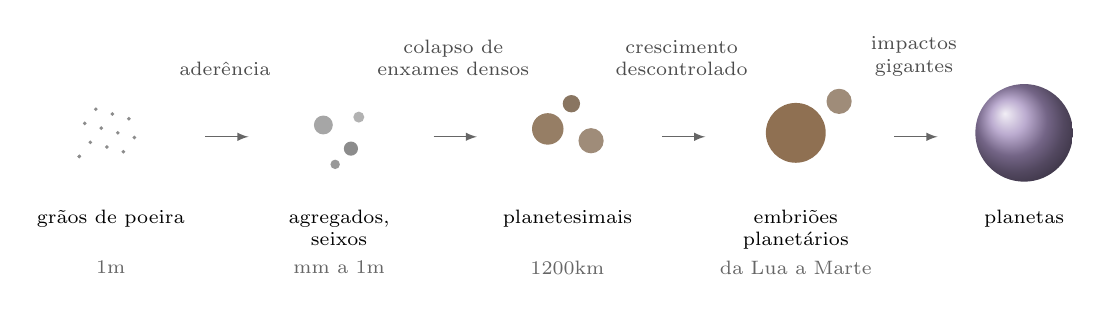
\begin{tikzpicture}[x=1cm, y=1cm, font=\scriptsize]
\foreach \x/\t/\s in {0/{grãos de poeira}/{\qty{1}{\micro m}},
  2.9/{agregados,\\seixos}/{mm a \qty{1}{m}},
  5.8/{planetesimais}/{\qtyrange{1}{200}{km}},
  8.7/{embriões\\planetários}/{da Lua a Marte},
  11.6/{planetas}/{} } {
  \node[align=center, anchor=north] at (\x,-0.9) {\t};
  \node[align=center, anchor=north, black!60] at (\x,-1.55) {\s};
}
\foreach \i in {0,...,11} {\fill[black!45] ({-0.4+0.07*mod(\i*7,11)},{-0.35+0.06*mod(\i*5,11)}) circle (0.025);}
\fill[black!35] (2.7,0.05) circle (0.12); \fill[black!45] (3.05,-0.25) circle (0.09);
\fill[black!40] (2.85,-0.45) circle (0.06); \fill[black!30] (3.15,0.15) circle (0.07);
\fill[brown!55!black!70] (5.55,0) circle (0.2); \fill[brown!50!black!60] (6.1,-0.15) circle (0.16);
\fill[brown!45!black!70] (5.85,0.32) circle (0.11);
\fill[brown!60!black!80] (8.7,-0.05) circle (0.38); \fill[brown!50!black!60] (9.25,0.35) circle (0.16);
\shade[ball color=blue!45!brown!60] (11.6,-0.05) circle (0.62);
\foreach \x in {1.2,4.1,7.0,9.95} {\draw[-latex, black!60] (\x,-0.1) -- +(0.55,0);}
\node[align=center, anchor=south, black!70] at (1.45,0.55) {aderência};
\node[align=center, anchor=south, black!70] at (4.35,0.55) {colapso de\\enxames densos};
\node[align=center, anchor=south, black!70] at (7.25,0.55) {crescimento\\descontrolado};
\node[align=center, anchor=south, black!70] at (10.2,0.55) {impactos\\gigantes};
\end{tikzpicture}

\par\smallskip{\small Da poeira aos planetas na região dos planetas rochosos
(esquema, fora de escala). Os grãos grudam em agregados; enxames de seixos colapsam
em \omterm{def:b2:planet-formation-meteorites:planetesimal}{planetesimais}; a gravidade faz alguns \omterm{def:b2:planet-formation-meteorites:planetesimal}{planetesimais} crescerem descontroladamente até virar embriões, que
acabam se fundindo em planetas. Além da \omterm{def:b2:planet-formation-meteorites:snow-line}{linha de neve}, os embriões cresceram mais e puderam
capturar gás. Tamanhos segundo Chiang e Youdin (2010) e Lugaro e colaboradores (2018).}
% ledger: cy10:growth, lugaro:cai
\end{omfigure}

Os planetas guardaram pouca memória dessa história: eles fundiram, misturaram e
retrabalharam sua matéria. O registro está nos corpos que pararam de crescer, os
asteroides, e nos fragmentos deles que chegam à Terra.

\section{Meteoritos}

\begin{definition}[Meteorito, queda, achado]
\label{def:b2:planet-formation-meteorites:fall-find}
Um \emph{meteorito}\index{meteorito} é um objeto sólido natural vindo do espaço que
sobreviveu à passagem pela atmosfera e chegou ao solo. Uma
\emph{queda}\index{queda} é um meteorito coletado depois que sua
chegada foi observada, em geral como uma bola de fogo; um
\emph{achado}\index{achado} é um meteorito reconhecido no solo sem que sua queda
tenha sido vista.
\end{definition}

A Terra recolhe muito mais poeira que pedras. Medido na neve do
planalto antártico, cerca de \qty{5200}{t} de poeira extraterrestre chegam ao
solo a cada ano como micrometeoritos e esférulas fundidas, de umas
\qty{15000}{t} que entram na atmosfera, a maior parte liberada por cometas e cerca de um
quinto por asteroides. Os \omterm{def:b2:planet-formation-meteorites:fall-find}{meteoritos}, as pedras e os ferros grandes o bastante para serem
reconhecidos um a um, são menos numerosos: o catálogo mundial contém cerca de
\num{45000}, dos quais apenas \num{1107} são \omterm{def:b2:planet-formation-meteorites:fall-find}{quedas}.
% ledger: rojas21:flux, data:b4-meteorites

A distinção é importante. Uma \omterm{def:b2:planet-formation-meteorites:fall-find}{queda} é coletada em poucos dias, antes que a chuva e o
oxigênio a alterem, e todos os tipos de \omterm{def:b2:planet-formation-meteorites:fall-find}{meteorito} que caem são coletados
da mesma forma; um \omterm{def:b2:planet-formation-meteorites:fall-find}{achado} pode ter ficado no solo por milhares de anos, e sua
chance de ser encontrado depende de sua aparência e de onde caiu. Metade de todos os
\omterm{def:b2:planet-formation-meteorites:fall-find}{achados} foi feita na Antártida (quadro abaixo), onde a busca é
sistemática. As \omterm{def:b2:planet-formation-meteorites:fall-find}{quedas} são a amostra mais fiel do que chega (figura abaixo):
mais de quatro em cada cinco são \omterm{def:b2:planet-formation-meteorites:chondrule}{condritos}, e três em cada quatro, \omterm{def:b2:planet-formation-meteorites:chondrule}{condritos} ordinários.
% ledger: data:b4-meteorites

\begin{omfigure}
\begin{tikzpicture}
\begin{axis}[width=0.86\linewidth, height=6.3cm, ybar, bar width=7pt,
  xmin=0.4, xmax=9.6, ymin=0.1, ymax=200, ymode=log, log origin=infty,
  xtick={1,...,9}, xticklabels={ordinários, carbonáceos, enstatíticos, outros condritos,
    HED, outros acondritos, ferrosos, metalo-rochosos, não classificados},
  x tick label style={font=\scriptsize, rotate=30, anchor=north east, inner sep=1pt},
  tick label style={font=\scriptsize}, label style={font=\small},
  ylabel={parcela da amostra (\%)}, legend pos=north east, xtick pos=bottom,
  legend style={font=\scriptsize, draw=black!30}, ymajorgrids, grid style={black!12}]
\addplot[fill=orange!70, draw=none] table[x=idx, y=falls_pct] {figdata/out/bachelor-2-meteorites-frac.dat};
\addlegendentry{quedas (\num{1107})}
\addplot[fill=blue!45, draw=none] table[x=idx, y=finds_pct] {figdata/out/bachelor-2-meteorites-frac.dat};
\addlegendentry{achados (\num{44534})}
\end{axis}
\end{tikzpicture}

\par\smallskip{\small \omterm{def:b2:planet-formation-meteorites:fall-find}{Meteoritos} por classe, em porcentagem das \omterm{def:b2:planet-formation-meteorites:fall-find}{quedas} e dos
\omterm{def:b2:planet-formation-meteorites:fall-find}{achados} (escala logarítmica); HED: howarditos, eucritos e diogenitos. Dados: exportação da NASA
da Meteoritical Bulletin Database da The Meteoritical Society
(\num{45641} \omterm{def:b2:planet-formation-meteorites:fall-find}{meteoritos} válidos).}
% ledger: data:b4-meteorites
\end{omfigure}

\begin{inthefield}[Em busca de meteoritos no gelo azul]
\begin{minipage}[t]{0.6\linewidth}\vspace{0pt}
A maior parte do manto de gelo antártico é neve branca, mas em cerca de
\qty{1}{\percent} de sua superfície, onde montanhas bloqueiam o fluxo do gelo,
cerca de \qty{5}{cm} de gelo se perdem a cada ano e o gelo azul fica exposto. Os \omterm{def:b2:planet-formation-meteorites:fall-find}{meteoritos}
que caíram sobre a neve a montante, ao longo de dezenas de milhares de anos, são soterrados,
transportados no gelo e trazidos de volta à superfície onde ele se consome:
o gelo azul é uma armadilha. Desde que a coleta sistemática começou, em meados da década de 1970,
equipes recuperaram mais de \num{30000} espécimes desses campos, e no
catálogo metade de todos os \omterm{def:b2:planet-formation-meteorites:fall-find}{achados} vem do sul de \ang{60}\,S. Os pesquisadores
atravessam o gelo em fileiras, a pé ou em motos de neve, e toda pedra encontrada é
coletada, por mais comum que pareça, para que a coleção não seja enviesada
em favor das mais chamativas. Cada \omterm{def:b2:planet-formation-meteorites:fall-find}{achado} é fotografado onde está, para registrar
seu contexto, e recebe um número de campo; mais tarde ele recebe seu nome oficial, um
código de três letras para o campo de gelo seguido do ano da temporada e de um
número de série. No laboratório de curadoria, as pedras são lascadas com
ferramentas de aço inoxidável ou cortadas a seco com uma serra de fita; os \omterm{def:b2:planet-formation-meteorites:chondrule}{condritos carbonáceos},
que podem conter compostos orgânicos, têm um gabinete só para eles desde 1978.
\end{minipage}\hfill
\begin{minipage}[t]{0.37\linewidth}\vspace{0pt}
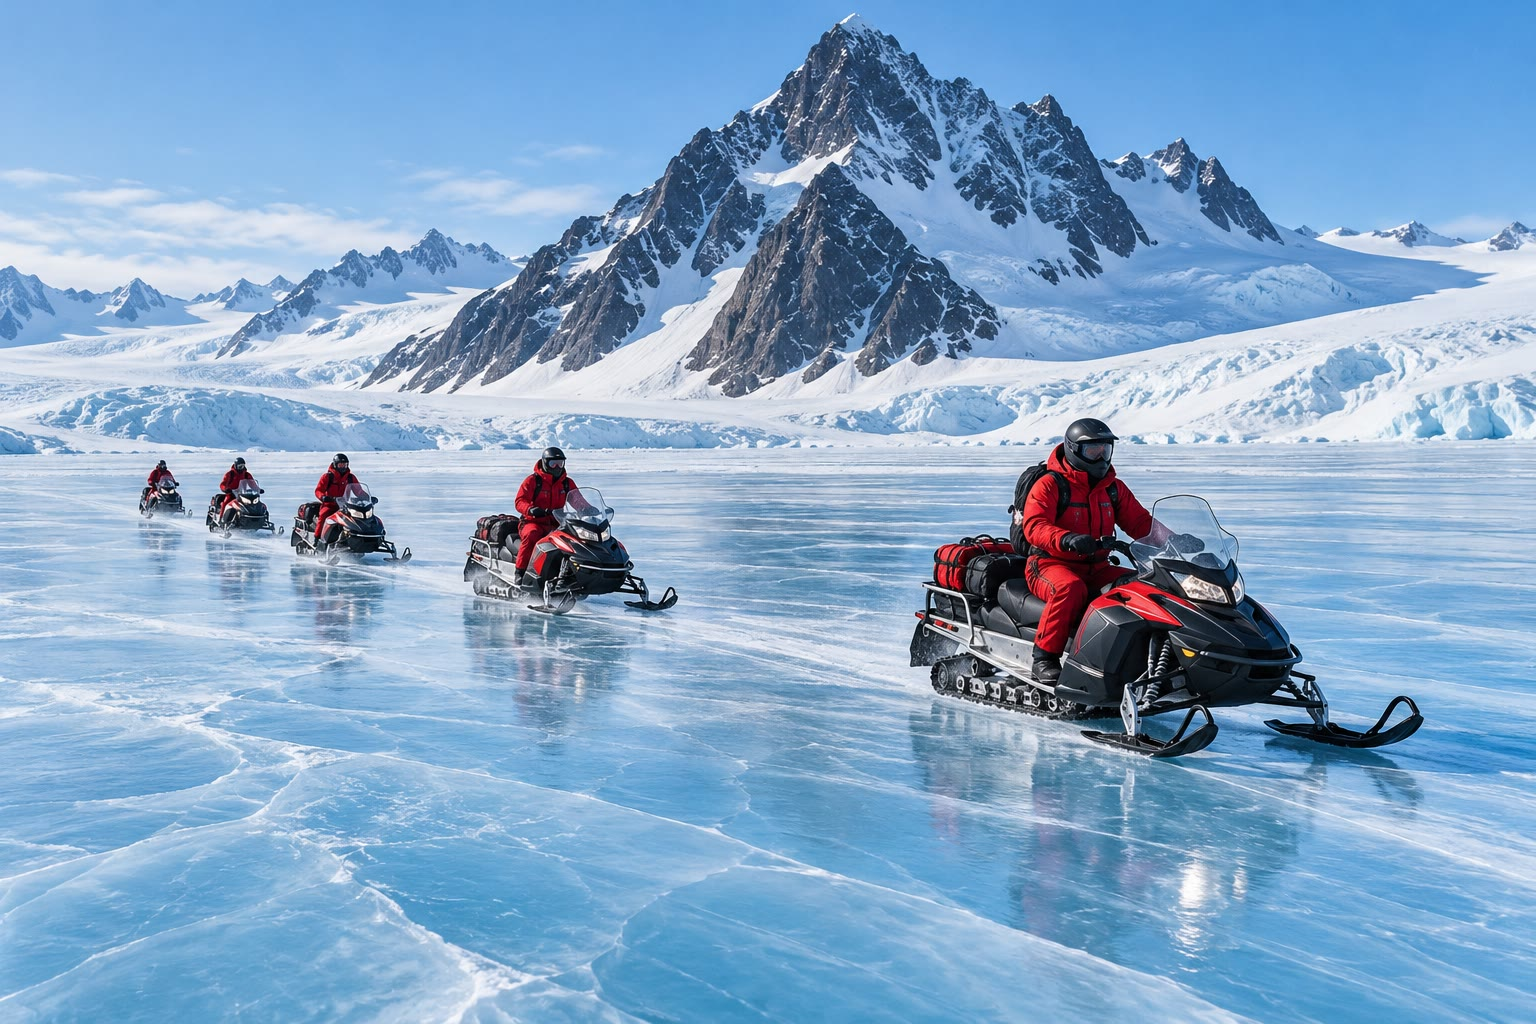
\includegraphics[width=\linewidth]{images/book4/ai/b2-blue-ice-search.jpg}

{\scriptsize Uma fileira de pesquisadores em motos de neve atravessando um campo de gelo azul abaixo de
um pico rochoso (ilustração gerada por IA).}
\end{minipage}
% ledger: folco06:blue-ice, data:b4-meteorites, nasa:antmet
\end{inthefield}

\subsection{Condritos}

\begin{definition}[Condrito, condrito carbonáceo, côndrulo, CAI]
\label{def:b2:planet-formation-meteorites:chondrule}
Um \emph{condrito}\index{condrito} é um \omterm{def:b2:planet-formation-meteorites:fall-find}{meteorito} rochoso que nunca fundiu
depois de agregado, e cuja composição, exceto pelos elementos mais voláteis,
é próxima da do Sol. A maior parte dele é feita de
\emph{côndrulos}\index{côndrulo}, gotículas arredondadas, de um décimo de milímetro a
cerca de um centímetro de diâmetro, de rocha silicática solidificada a partir de um fundido, imersas em
uma matriz de grão fino com grãos de metal ferro--níquel e sulfeto de ferro. Alguns
condritos contêm \emph{inclusões ricas em cálcio e alumínio}\index{inclusão rica em cálcio e alumínio}
(CAIs), grãos brancos irregulares de minerais de cálcio, alumínio
e titânio que são os primeiros condensados da nebulosa. Um
\emph{condrito carbonáceo}\index{condrito carbonáceo} é um condrito rico
em carbono, em minerais hidratados e em matriz, cujo teor de elementos voláteis
é o mais próximo do do Sol.
\end{definition}

Os \omterm{def:b2:planet-formation-meteorites:chondrule}{côndrulos} ficaram fundidos por apenas minutos e esfriaram em horas ou
dias: um aquecimento breve, local e súbito na nebulosa, de causa ainda
desconhecida, fundiu aglomerados de poeira, que se solidificaram como gotículas antes de serem varridos,
junto com poeira e metal, para um \omterm{def:b2:planet-formation-meteorites:planetesimal}{planetesimal}. Eles ocupam até \qty{90}{\percent} do volume dos \omterm{def:b2:planet-formation-meteorites:fall-find}{meteoritos} mais
primitivos. As CAIs representam de menos de \qty{1}{\percent} dos
\omterm{def:b2:planet-formation-meteorites:chondrule}{condritos} ordinários a mais de \qty{10}{\percent} de alguns carbonáceos, e elas
se formaram com no máximo cerca de cem mil anos de diferença entre si.
% ledger: gail:meteorites, cy10:growth, cy10:chondrules, gail:chondrite-table, lugaro:cai

\begin{omfigure}
\begin{minipage}[c]{0.5\linewidth}
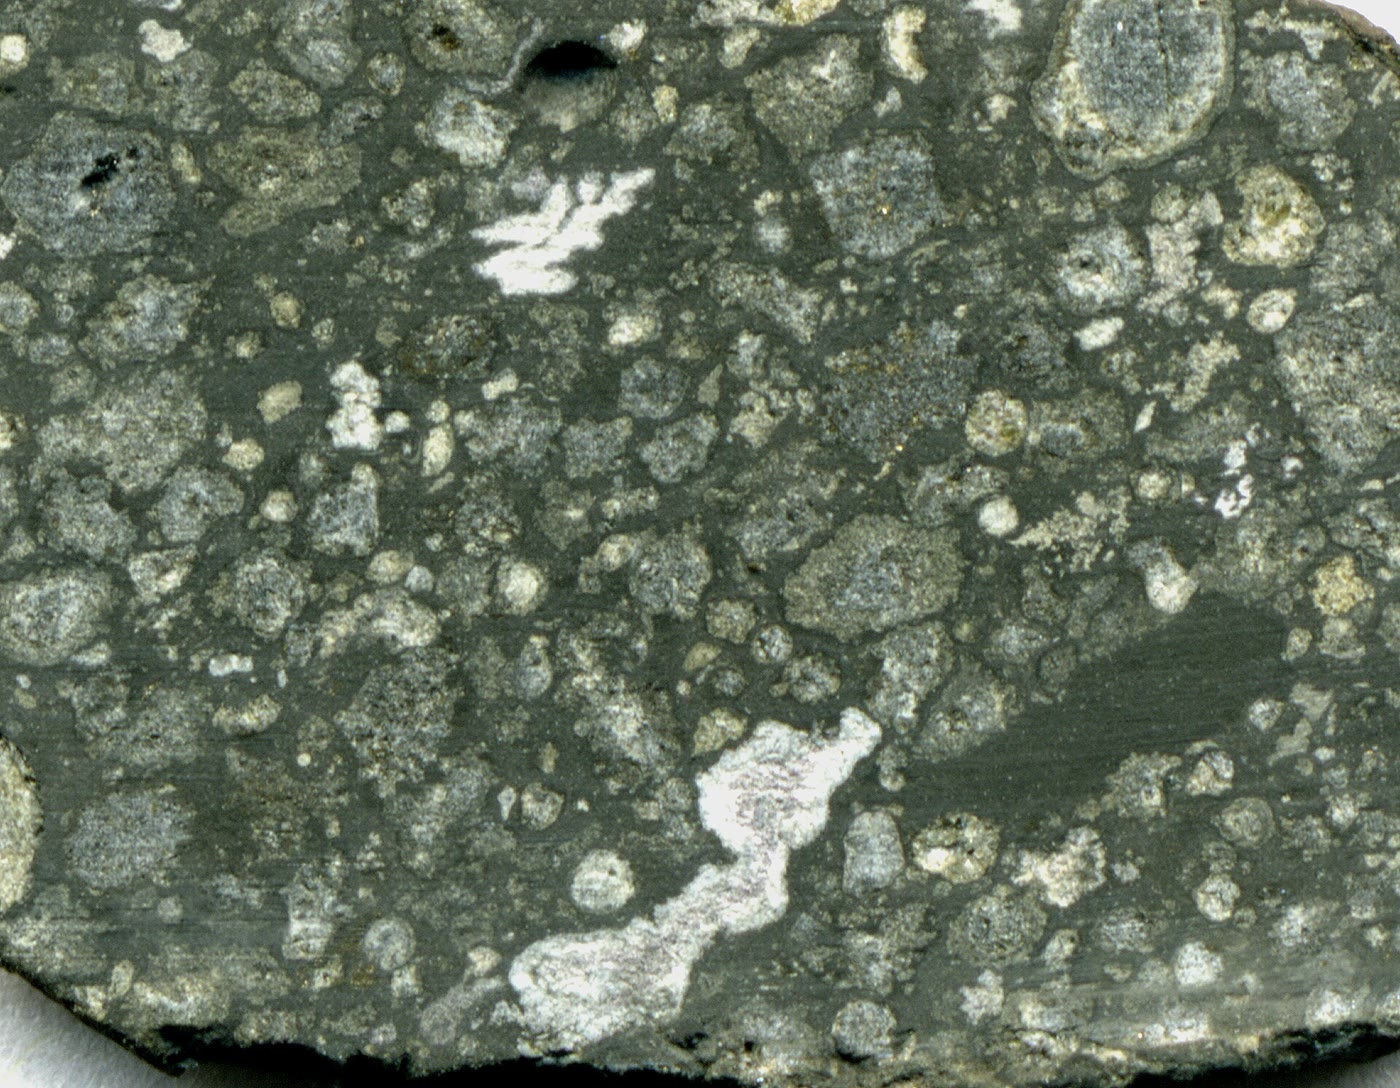
\includegraphics[width=\linewidth]{images/book4/b2-allende-chondrite.jpg}
\end{minipage}\hfill
\begin{minipage}[c]{0.46\linewidth}
{\small Uma face cortada do \omterm{def:b2:planet-formation-meteorites:chondrule}{condrito carbonáceo} Allende (classe CV3), que caiu no
norte do México em 1969: cerca de duas toneladas foram coletadas. Os grãos cinza arredondados são
\omterm{def:b2:planet-formation-meteorites:chondrule}{côndrulos}; as manchas brancas irregulares são CAIs; o cimento escuro é a matriz. O
campo tem alguns centímetros de largura. James St.\ John, CC BY 2.0.}
\end{minipage}
% ledger: data:b4-meteorites, gail:chondrite-table
\end{omfigure}

Os \omterm{def:b2:planet-formation-meteorites:chondrule}{condritos} se dividem em grupos que diferem no tamanho e na abundância de seus
\omterm{def:b2:planet-formation-meteorites:chondrule}{côndrulos}, em seu teor de metal, no teor de ferro de sua olivina e na
proporção de sua matriz (tabela abaixo). Os \omterm{def:b2:planet-formation-meteorites:chondrule}{condritos} ordinários H, L e LL
têm teores altos, baixos e muito baixos de metal e de ferro total (razões atômicas
Fe/Si de \num{0.80}, \num{0.59} e \num{0.53}).
% ledger: gail:chondrite-table

\begin{table}[h]
\centering
\small
\begin{tabular}{lcccccc}
\hline
 & H & L & LL & CI & CM & CV\\
\hline
\omterm{def:b2:planet-formation-meteorites:chondrule}{côndrulos} (vol.\ \%) & 60--80 & 60--80 & 60--80 & $\ll 1$ & 20 & 45\\
diâmetro médio dos \omterm{def:b2:planet-formation-meteorites:chondrule}{côndrulos} (mm) & 0.3 & 0.7 & 0.9 & --- & 0.3 & 1.0\\
CAIs (vol.\ \%) & 0.1--1 & 0.1--1 & 0.1--1 & $\ll 1$ & 5 & 10\\
matriz (vol.\ \%) & 10--15 & 10--15 & 10--15 & $> 99$ & 70 & 40\\
metal ferro--níquel (vol.\ \%) & 10 & 5 & 2 & 0 & 0.1 & 0--5\\
faialita na olivina (mol \%) & 16--20 & 23--26 & 27--32 & & & \\
\omterm{def:b2:planet-formation-meteorites:type}{tipos petrológicos} & 3--6 & 3--6 & 3--6 & 1 & 2 & 3\\
temperatura máxima (K) & 1220 & 1220 & 1220 & 430 & 670 & 870\\
\hline
\end{tabular}
\caption{Propriedades dos \omterm{def:b2:planet-formation-meteorites:chondrule}{condritos} ordinários (H, L, LL) e de três grupos de \omterm{def:b2:planet-formation-meteorites:chondrule}{condritos
carbonáceos}. Faialita: o membro extremo ferroso da olivina. Dados: Gail e colaboradores (2014).}
\label{tab:b2:planet-formation-meteorites:chondrites}
% ledger: gail:chondrite-table
\end{table}

\begin{definition}[Tipo petrológico]\label{def:b2:planet-formation-meteorites:type}
O \emph{tipo petrológico}\index{tipo petrológico} de um \omterm{def:b2:planet-formation-meteorites:chondrule}{condrito} é um número
de 1 a 6 que registra o que lhe aconteceu em seu corpo parental: o tipo 3 é o
menos alterado; os tipos 4 a 6 são cada vez mais aquecidos, com \omterm{def:b2:planet-formation-meteorites:chondrule}{côndrulos} esmaecidos
e minerais recristalizados e de composição uniforme; os tipos 2 e 1 são
cada vez mais alterados pela água líquida, que transformou seus minerais em argilas.
\end{definition}

A última linha da tabela dá as temperaturas máximas atingidas por cada grupo:
até cerca de \qty{1220}{K} para os \omterm{def:b2:planet-formation-meteorites:chondrule}{condritos} ordinários mais aquecidos, nunca mais
de \qty{430}{K} para os \omterm{def:b2:planet-formation-meteorites:chondrule}{condritos} CI, encharcados de água, mas nunca quentes. O
aquecimento, como mostra a última seção, veio do interior dos corpos parentais.
% ledger: gail:chondrite-table

\subsection{Acondritos e meteoritos ferrosos}

\begin{definition}[Acondrito, meteorito ferroso, meteorito metalo-rochoso]
\label{def:b2:planet-formation-meteorites:classes}
Um \emph{acondrito}\index{acondrito} é um \omterm{def:b2:planet-formation-meteorites:fall-find}{meteorito} rochoso que cristalizou
a partir de um fundido ou recristalizou a alta temperatura em um corpo que fundiu, e
por isso não tem \omterm{def:b2:planet-formation-meteorites:chondrule}{côndrulos}. Um \emph{meteorito ferroso}\index{meteorito ferroso} é feito
principalmente de metal ferro--níquel. Um \emph{meteorito
metalo-rochoso}\index{meteorito metalo-rochoso} é feito de metal e silicato em quantidades
aproximadamente iguais.
\end{definition}

Eles são os fragmentos de corpos que fundiram e se diferenciaram: os \omterm{def:b2:planet-formation-meteorites:classes}{acondritos} são suas
crostas e mantos, os ferrosos, seus núcleos metálicos, e os metalo-rochosos vêm do lugar onde
metal e silicato se encontravam. A maior família de \omterm{def:b2:planet-formation-meteorites:classes}{acondritos}, a dos howarditos,
eucritos e diogenitos (HED), basaltos e rochas ricas em piroxênio, representa
\qty{5.5}{\percent} de todas as \omterm{def:b2:planet-formation-meteorites:fall-find}{quedas}. Sua fonte foi identificada, por seu espectro e
sua órbita, como o asteroide Vesta, com cerca de \qty{525}{km} de diâmetro, e a sonda Dawn,
que chegou a Vesta em 2011, confirmou isso: a química
e a mineralogia da superfície de Vesta correspondem às dos \omterm{def:b2:planet-formation-meteorites:fall-find}{meteoritos} HED, uma bacia
de \qty{500}{km} de largura perto de seu polo sul mostra de onde os fragmentos foram
arrancados, e seu campo de gravidade indica um núcleo de ferro de cerca de \qty{225}{km} de diâmetro.
Vesta fundiu, quase ou totalmente, no início de sua história. Outros \omterm{def:b2:planet-formation-meteorites:classes}{acondritos} vêm
da Lua e de Marte. Os \omterm{def:b2:planet-formation-meteorites:fall-find}{meteoritos} das coleções parecem vir
de cerca de cem corpos parentais diferentes.
% ledger: data:b4-meteorites, nasa:vesta-dawn, gail:meteorites

Os \omterm{def:b2:planet-formation-meteorites:classes}{meteoritos ferrosos} guardam o registro de como seus núcleos esfriaram. Uma face cortada e
atacada por ácido mostra um entrecruzado de placas (figura abaixo): a alta
temperatura, o metal é uma única liga de ferro e níquel; com o resfriamento lento, uma
liga pobre em níquel cresce em placas ao longo dos planos do cristal original,
e quanto mais lento o resfriamento, mais largas as placas. Medidas em muitos \omterm{def:b2:planet-formation-meteorites:classes}{meteoritos ferrosos}, as
larguras das placas dão as taxas de resfriamento dos núcleos de onde eles vieram.
% ledger: gail:meteorites

\begin{omfigure}
\begin{minipage}[c]{0.5\linewidth}
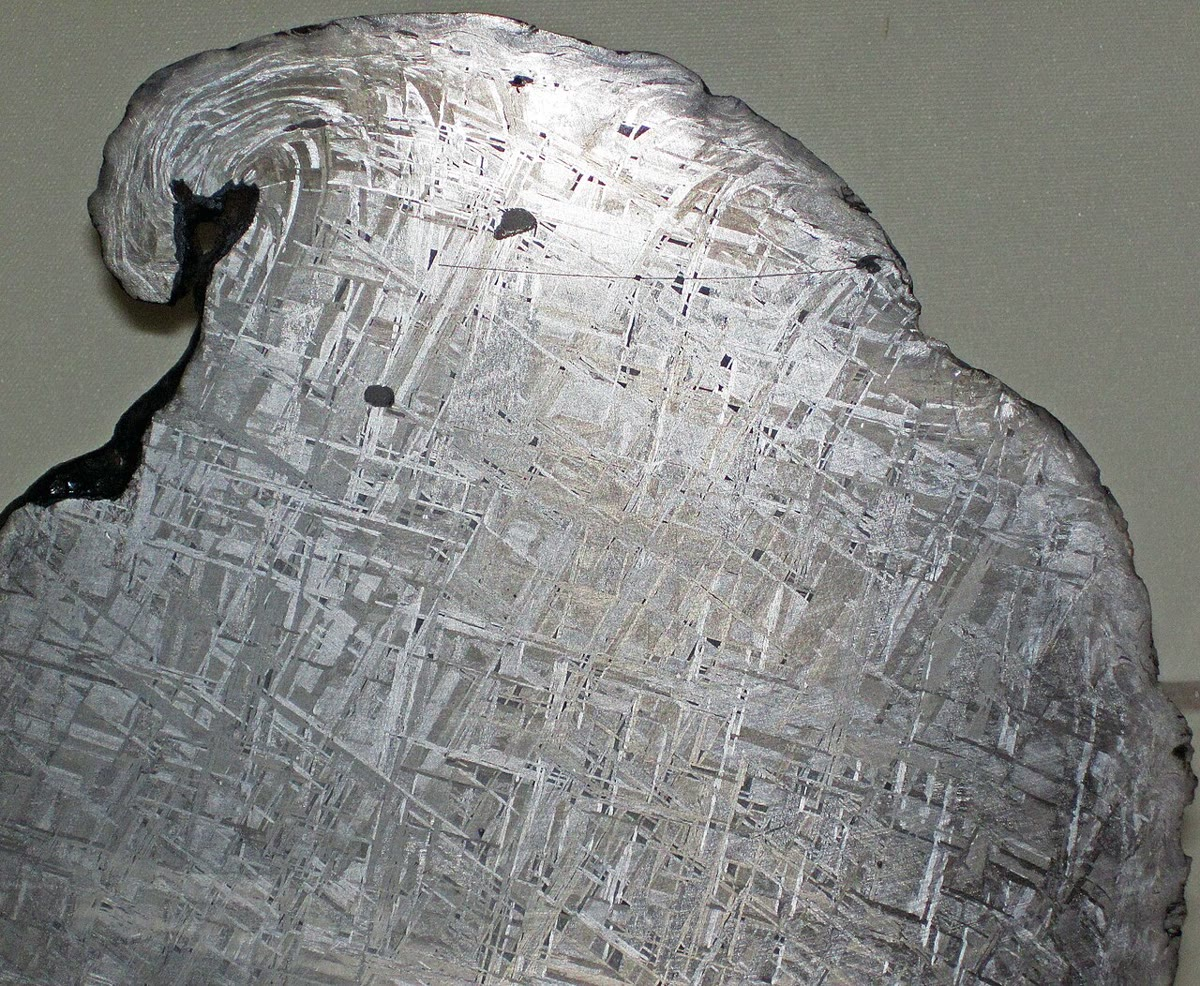
\includegraphics[width=\linewidth]{images/book4/b2-gibeon-widmanstatten.jpg}
\end{minipage}\hfill
\begin{minipage}[c]{0.46\linewidth}
{\small A face cortada, polida e atacada por ácido de um fragmento do \omterm{def:b2:planet-formation-meteorites:classes}{meteorito ferroso} Gibeon,
encontrado na Namíbia: o entrecruzado de placas de liga ferro--níquel (o padrão de
Widmanstätten) cresceu enquanto o núcleo metálico de seu corpo parental esfriava lentamente. James St.\ John,
CC BY 2.0.}
\end{minipage}
% ledger: data:b4-meteorites
\end{omfigure}

\section{Datando o Sistema Solar}

A idade do Sistema Solar é a idade de seus sólidos mais antigos. As isócronas
urânio--chumbo das CAIs, construídas como no volume do primeiro ano, dão \qtyrange{4567}{4568}{\Ma};
as CAIs se formaram com no máximo cerca de \qty{0.1}{Myr} de diferença entre si, um tempo curto
o bastante para que sua idade seja tomada como o nascimento do Sol. Os acontecimentos dos
poucos milhões de anos seguintes, a formação dos \omterm{def:b2:planet-formation-meteorites:chondrule}{côndrulos} e a agregação e a
fusão dos primeiros corpos, são mais bem datados em relação às CAIs, com relógios
que corriam depressa e pararam cedo.
% ledger: lugaro:cai

\begin{definition}[Radionuclídeo de vida curta]
\label{def:b2:planet-formation-meteorites:slr}
Um \emph{radionuclídeo de vida curta}\index{radionuclídeo de vida curta} é um
nuclídeo radioativo com meia-vida de aproximadamente \num{0.1} a \qty{100}{Myr},
presente quando o Sistema Solar se formou e hoje extinto, cuja presença passada
é revelada por um excesso de seu filho em minerais que eram ricos em seu
elemento.
\end{definition}

O mais conhecido é o alumínio-26, que decai em magnésio-26 com meia-vida de
\qty{0.717}{Myr} (vida média de \qty{1.035}{Myr}). Quando as CAIs se formaram, um
átomo de alumínio em cerca de \num{19000} era alumínio-26: a razão
$\ce{^{26}Al}/\ce{^{27}Al}$ era $(5.23 \pm 0.13)\times10^{-5}$, o valor
\emph{canônico}. Outros nuclídeos de vida curta cobrem intervalos mais longos (tabela
abaixo).
% ledger: lugaro:al26, lugaro:slr-table

\begin{table}[h]
\centering
\small
\begin{tabular}{lllcc}
\hline
nuclídeo & filho & referência & meia-vida (Myr) & razão inicial\\
\hline
\ce{^{26}Al} & \ce{^{26}Mg} & \ce{^{27}Al} & 0.717 & $5.23\times10^{-5}$\\
\ce{^{60}Fe} & \ce{^{60}Ni} & \ce{^{56}Fe} & 2.62 & $1.0\times10^{-8}$\\
\ce{^{53}Mn} & \ce{^{53}Cr} & \ce{^{55}Mn} & 3.74 & $7\times10^{-6}$\\
\ce{^{107}Pd} & \ce{^{107}Ag} & \ce{^{108}Pd} & 6.5 & $6.6\times10^{-5}$\\
\ce{^{182}Hf} & \ce{^{182}W} & \ce{^{180}Hf} & 8.90 & $1.02\times10^{-4}$\\
\ce{^{129}I} & \ce{^{129}Xe} & \ce{^{127}I} & 15.7 & $1.28\times10^{-4}$\\
\hline
\end{tabular}
\caption{Alguns \omterm{def:b2:planet-formation-meteorites:slr}{radionuclídeos de vida curta} do Sistema Solar primitivo, seu filho
estável, o isótopo estável do mesmo elemento usado como referência, sua
meia-vida e sua razão em relação à referência quando as CAIs se formaram. Dados: Lugaro e
colaboradores (2018).}
\label{tab:b2:planet-formation-meteorites:slr}
% ledger: lugaro:al26, lugaro:slr-table
\end{table}

\begin{proposition}[Idade relativa a partir de um nuclídeo extinto]
\label{prop:b2:planet-formation-meteorites:relative-age}
Se a razão entre um nuclídeo de vida curta e seu isótopo de referência era $R_0$
em toda parte quando as CAIs se formaram, e se constata que ela era $R$ em um objeto quando
ele se formou, o objeto se formou
\[
  \Delta t = \tau \ln\frac{R_0}{R}
\]
depois das CAIs, em que $\tau$ é a vida média do nuclídeo. Um erro
$\delta R$ em $R$ dá o erro $\tau\,\delta R/R$ em $\Delta t$.
\end{proposition}

\begin{proof}
O isótopo de referência é estável, de modo que a razão decai como o próprio nuclídeo
radioativo: $R = R_0 e^{-\Delta t/\tau}$. Tomando logaritmos,
$\Delta t = \tau\ln(R_0/R)$. Diferenciando, $\mathrm d(\Delta t) =
-\tau\,\mathrm dR/R$.
\end{proof}

Um erro relativo de \qty{10}{\percent} na razão custa, assim,
\qty{0.1}{Myr} com o alumínio-26, mas \qty{0.54}{Myr} com o manganês-53 e
\qty{1.3}{Myr} com o háfnio-182: cada relógio só é preciso ao longo de algumas de suas
próprias vidas médias, e o relógio certo depende do acontecimento. A razão $R$ em um
objeto é lida em seus minerais.
% ledger: lugaro:al26, lugaro:slr-table

\begin{proposition}[Isócrona alumínio--magnésio]
\label{prop:b2:planet-formation-meteorites:al-mg}
Sejam vários minerais de um mesmo objeto formados juntos no instante $\Delta t$ com a
mesma composição isotópica do magnésio, $(\ce{^{26}Mg}/\ce{^{24}Mg})_0$, mas
razões $\ce{^{27}Al}/\ce{^{24}Mg}$ diferentes, e fechados desde então. Hoje eles
ficam sobre a reta
\[
  \frac{\ce{^{26}Mg}}{\ce{^{24}Mg}}
  = \left(\frac{\ce{^{26}Mg}}{\ce{^{24}Mg}}\right)_0
  + R\,\frac{\ce{^{27}Al}}{\ce{^{24}Mg}},
\]
cuja inclinação é a razão $R = \ce{^{26}Al}/\ce{^{27}Al}$ do objeto quando ele
se formou.
\end{proposition}

\begin{proof}
Todo átomo de alumínio-26 presente na formação tornou-se desde então um
átomo de magnésio-26, de modo que um mineral ganhou
$\ce{^{26}Al}_{\text{inicial}} = R\,\ce{^{27}Al}$ átomos de magnésio-26, sendo o alumínio-27
estável. Dividir pelo número de átomos de magnésio-24, que não muda,
dá a reta.
\end{proof}

Os minerais ricos em alumínio e pobres em magnésio, como o plagioclásio, mostram grandes excessos
de magnésio-26; a olivina, quase sem alumínio, não mostra nenhum. Foi assim que se
construiu a sequência temporal do Sistema Solar primitivo: primeiro as CAIs; os \omterm{def:b2:planet-formation-meteorites:chondrule}{côndrulos} ao longo
dos poucos milhões de anos seguintes, com os indícios dos \omterm{def:b2:planet-formation-meteorites:chondrule}{côndrulos} fixando a
duração de vida do disco de gás em menos de cinco milhões de anos; os corpos parentais
dos \omterm{def:b2:planet-formation-meteorites:chondrule}{condritos} agregados depois de seus \omterm{def:b2:planet-formation-meteorites:chondrule}{côndrulos} mais jovens. Os diogenitos,
rochas do manto de Vesta, começaram a cristalizar cerca de um milhão de anos depois
das CAIs, e o núcleo de Vesta se formou entre o primeiro e o
quarto milhão de anos: os \omterm{def:b2:planet-formation-meteorites:classes}{meteoritos ferrosos} e os \omterm{def:b2:planet-formation-meteorites:classes}{acondritos} são mais velhos que muitos
\omterm{def:b2:planet-formation-meteorites:chondrule}{condritos}.
% ledger: lugaro:cai, gail:vesta, gail:meteorites

\section{O calor do alumínio-26 e as primeiras fusões}

De onde veio o calor que fundiu Vesta e metamorfizou os \omterm{def:b2:planet-formation-meteorites:chondrule}{condritos}
ordinários? Modelos e \omterm{def:b2:planet-formation-meteorites:fall-find}{meteoritos} concordam que, nos corpos mais antigos,
a fonte dominante foi o decaimento do alumínio-26. Em uma rocha de composição condrítica, ele trazia, no início,
\qty{5}{MJ} por quilograma prontos para serem liberados em poucos milhões de anos:
o suficiente para aquecer a rocha em milhares de kelvins, se o calor não pudesse escapar.
% ledger: lugaro:heat, lugaro:melting

\begin{proposition}[Aquecimento de um planetesimal pelo alumínio-26]
\label{prop:b2:planet-formation-meteorites:heating}
Uma rocha que recebe a potência radioativa $H_0 e^{-t/\tau}$ por quilograma, que tem
a capacidade térmica específica $c$ e não perde calor, aquece-se depois de sua acreção no
instante $t_a$ segundo
\[
  T(t) = T_0 + \frac{H_0\tau}{c}\left(e^{-t_a/\tau} - e^{-t/\tau}\right),
\]
e tende para a temperatura máxima
$T_{\max} = T_0 + (H_0\tau/c)\,e^{-t_a/\tau}$. Uma temperatura crítica
$T_c > T_0$ só é atingida se o corpo se agregou antes de
\[
  t_a^* = \tau\ln\frac{H_0\tau}{c\,(T_c - T_0)}.
\]
\end{proposition}

\begin{proof}
Sem perdas, $c\,\mathrm dT/\mathrm dt = H_0 e^{-t/\tau}$. Integrar a partir de
$t_a$, em que $T = T_0$, dá
$c\,(T - T_0) = H_0\tau\,(e^{-t_a/\tau} - e^{-t/\tau})$, que tende para
$H_0\tau e^{-t_a/\tau}$ quando $t \to \infty$. Fazer $T_{\max} = T_c$ e resolver
para $t_a$ dá $t_a^*$; para uma acreção mais precoce, o máximo é mais alto.
\end{proof}

Um modelo do corpo parental dos \omterm{def:b2:planet-formation-meteorites:chondrule}{condritos} ordinários usa
$H_0 = \qty{1.9e-7}{W.kg^{-1}}$, $c = \qty{837}{J.kg^{-1}.K^{-1}}$ e
$T_0 = \qty{250}{K}$. Então $H_0\tau/c$ vale cerca de \qty{7400}{K}. Três
temperaturas importam: perto de \qty{750}{K}, a rocha porosa começa a sinterizar e se torna
compacta; perto de \qty{1200}{K}, o metal e o sulfeto de ferro começam a fundir
juntos; perto de \qty{1700}{K}, os últimos silicatos fundem. Um corpo que se agregou
antes de \qty{1.7}{Myr} fundiu inteiramente; antes de \qty{2.1}{Myr}, seu metal e seu sulfeto
fundiram e puderam afundar formando um núcleo; até cerca de \qty{2.8}{Myr}, ele foi pelo menos
sinterizado e metamorfizado; os corpos posteriores permaneceram frios (figura abaixo).
% ledger: gail:params, gail:temps, lugaro:al26

\begin{omfigure}
\begin{tikzpicture}
\begin{axis}[omrecord, name=left, width=0.45\linewidth, height=6.0cm,
  xmin=0, xmax=8, ymin=0, ymax=2300,
  xlabel={tempo depois das CAIs (Myr)}, ylabel={temperatura (K)},
  tick label style={font=\scriptsize}, label style={font=\small}]
\addplot[black!45, densely dashed, domain=0:8, samples=2] {750};
\addplot[black!45, densely dashed, domain=0:8, samples=2] {1200};
\addplot[black!45, densely dashed, domain=0:8, samples=2] {1700};
\addplot[thick, red!75!black] table[x=t_Myr, y=T_K] {figdata/out/bachelor-2-al26-ta15.dat};
\addplot[thick, orange!80!black] table[x=t_Myr, y=T_K] {figdata/out/bachelor-2-al26-ta20.dat};
\addplot[thick, teal!70!black] table[x=t_Myr, y=T_K] {figdata/out/bachelor-2-al26-ta25.dat};
\addplot[thick, blue!70!black] table[x=t_Myr, y=T_K] {figdata/out/bachelor-2-al26-ta30.dat};
\node[font=\tiny, red!75!black, anchor=south east] at (axis cs:7.9,1995) {$t_a = \qty{1.5}{Myr}$};
\node[font=\tiny, orange!80!black, anchor=south east] at (axis cs:7.9,1325) {2};
\node[font=\tiny, teal!70!black, anchor=south east] at (axis cs:7.9,915) {2.5};
\node[font=\tiny, blue!70!black, anchor=north east] at (axis cs:7.9,650) {3};
\node[font=\tiny, black!60, anchor=south west] at (axis cs:0.1,1700) {silicatos fundidos};
\node[font=\tiny, black!60, anchor=south west] at (axis cs:0.1,1200) {Fe--FeS funde};
\node[font=\tiny, black!60, anchor=south west] at (axis cs:0.1,750) {sinterização};
\end{axis}
\begin{axis}[omrecord, at={(left.east)}, anchor=west, xshift=2.1cm, width=0.45\linewidth,
  height=6.0cm, xmin=0, xmax=4, ymin=0, ymax=8000,
  xlabel={tempo de acreção $t_a$ (Myr)}, ylabel={temperatura máxima (K)},
  tick label style={font=\scriptsize}, label style={font=\small},
  scaled y ticks=false, yticklabel style={/pgf/number format/1000 sep={\,}}]
\addplot[black!45, densely dashed, domain=0:4, samples=2] {750};
\addplot[black!45, densely dashed, domain=0:4, samples=2] {1200};
\addplot[black!45, densely dashed, domain=0:4, samples=2] {1700};
\addplot[thick, black] table[x=ta_Myr, y=Tpeak_K] {figdata/out/bachelor-2-al26-peak.dat};
\draw[black!60] (axis cs:1.69,0) -- (axis cs:1.69,1700);
\draw[black!60] (axis cs:2.13,0) -- (axis cs:2.13,1200);
\node[font=\tiny, black!70, anchor=south] at (axis cs:2.0,4500) {\qty{1.7}{Myr}};
\draw[black!50, -latex] (axis cs:2.0,4450) -- (axis cs:1.71,1800);
\node[font=\tiny, black!70, anchor=south] at (axis cs:2.9,3300) {\qty{2.1}{Myr}};
\draw[black!50, -latex] (axis cs:2.9,3250) -- (axis cs:2.16,1300);
\end{axis}
\end{tikzpicture}

\par\smallskip{\small Aquecimento pelo alumínio-26 do interior de um corpo condrítico sem
perda de calor (a proposição acima; $H_0 = \qty{1.9e-7}{W.kg^{-1}}$,
$c = \qty{837}{J.kg^{-1}.K^{-1}}$, $T_0 = \qty{250}{K}$, $\tau = \qty{1.035}{Myr}$).
À esquerda: temperatura em função do tempo para corpos agregados 1.5, 2, 2.5 e \qty{3}{Myr}
depois das CAIs. À direita: temperatura máxima em função do tempo de acreção; os corpos agregados
antes de \qty{1.7}{Myr} fundiram, e, antes de \qty{2.1}{Myr}, seu metal e seu sulfeto fundiram.
Os corpos reais gastam parte do calor na fusão, o que limita a temperatura, e perdem
calor perto da superfície. Valores do modelo: Gail e colaboradores (2014).}
% ledger: gail:params, gail:temps, lugaro:al26
\end{omfigure}

A proposição ignora a perda de calor, o que só é válido no interior profundo de um corpo grande.
O calor se difunde na distância $\sqrt{\kappa t}$ no tempo $t$, em que
$\kappa$ é a difusividade térmica da rocha: com os valores do modelo,
cerca de \qty{5}{km} em uma vida média do alumínio-26 (\cref{exo:b2:planet-formation-meteorites:12}). Os corpos muito
menores que isso perdem seu calor tão depressa quanto o produzem; modelos detalhados mostram
que corpos de mais de \qtyrange{10}{20}{km} de diâmetro podiam fundir.
% ledger: gail:params, lugaro:melting

\begin{definition}[Diferenciação planetária]
\label{def:b2:planet-formation-meteorites:differentiation}
A \emph{diferenciação planetária}\index{diferenciação planetária} é a
separação de um corpo, depois de fundido total ou parcialmente, em camadas de
composição e densidade diferentes: um núcleo metálico, um manto silicático e uma crosta feita
dos últimos fundidos.
\end{definition}

Os \omterm{def:b2:planet-formation-meteorites:fall-find}{meteoritos} registram, assim, dois tipos de corpos primitivos. Os que se formaram nos
primeiros dois milhões de anos, aproximadamente, tinham alumínio-26 suficiente para fundir e
se diferenciar: seus núcleos são os \omterm{def:b2:planet-formation-meteorites:classes}{meteoritos ferrosos}, suas crostas e mantos,
os \omterm{def:b2:planet-formation-meteorites:classes}{acondritos}, e Vesta é o sobrevivente. Os que se formaram mais tarde permaneceram
\omterm{def:b2:planet-formation-meteorites:chondrule}{condritos}, aquecidos por dentro em um grau fixado por sua data de nascimento e pela
profundidade de cada fragmento: os mais profundos tornaram-se tipo 6, os mais rasos permaneceram
tipo 3. A própria Terra, construída a partir de embriões e \omterm{def:b2:planet-formation-meteorites:planetesimal}{planetesimais} dos dois tipos e
atingida por impactos gigantes, diferenciou-se em núcleo, manto e crosta.
% ledger: gail:meteorites, gail:vesta, gail:temps

\section{Exercícios}

\begin{exercise}[$\star$]\label{exo:b2:planet-formation-meteorites:1}
Na \omterm{def:b2:planet-formation-meteorites:nebula}{nebulosa solar} de massa mínima, calcule a densidade superficial do gás a
\qty{1}{au} e a \qty{5.2}{au}, e a densidade superficial dos sólidos a
\qty{1}{au} (só rocha, $Z_{\mathrm{rel}} = 0.33$) e a \qty{5.2}{au} (todos os gelos
condensados, $Z_{\mathrm{rel}} = 1$). Quantas vezes mais pesado que os sólidos é o
gás a \qty{5.2}{au}?
% ledger: cy10:mmsn
\end{exercise}

\begin{exercise}[$\star$]\label{exo:b2:planet-formation-meteorites:2}
Usando a figura das \omterm{def:b2:planet-formation-meteorites:condensation}{temperaturas de condensação}, ordene o alumínio, o sódio,
o magnésio, o ferro, o enxofre e o oxigênio (como gelo de água) do primeiro a se condensar
ao último, e dê o grupo de volatilidade de cada um. Quais deles você esperaria
encontrar enriquecidos nas CAIs, e quais empobrecidos na Terra em comparação com o Sol?
% ledger: lodders:tc-table, lodders:groups
\end{exercise}

\begin{exercise}[$\star$]\label{exo:b2:planet-formation-meteorites:3}
O catálogo lista \num{1107} \omterm{def:b2:planet-formation-meteorites:fall-find}{quedas}, das quais 856 são \omterm{def:b2:planet-formation-meteorites:chondrule}{condritos} ordinários e
49 ferrosos, e \num{44534} \omterm{def:b2:planet-formation-meteorites:fall-find}{achados}, dos quais \num{38647} são \omterm{def:b2:planet-formation-meteorites:chondrule}{condritos} ordinários,
\num{1020} ferrosos e \num{22096} vêm do sul de \ang{60}\,S. Calcule a
parcela de \omterm{def:b2:planet-formation-meteorites:chondrule}{condritos} ordinários e de ferrosos entre as \omterm{def:b2:planet-formation-meteorites:fall-find}{quedas} e entre os \omterm{def:b2:planet-formation-meteorites:fall-find}{achados},
e a parcela de \omterm{def:b2:planet-formation-meteorites:fall-find}{achados} antárticos. Que amostra você usaria para estimar as
proporções em que as classes chegam à Terra, e por quê?
% ledger: data:b4-meteorites
\end{exercise}

\begin{exercise}[$\star$]\label{exo:b2:planet-formation-meteorites:4}
Os minerais de um objeto dão a razão inicial
$\ce{^{26}Al}/\ce{^{27}Al} = \num{1.0e-5}$. Quanto tempo depois das CAIs ele se formou?
Tome $R_0 = \num{5.23e-5}$ e uma vida média de \qty{1.035}{Myr}.
% ledger: lugaro:al26
\end{exercise}

\begin{exercise}[$\star\star$]\label{exo:b2:planet-formation-meteorites:5}
Usando a \cref{prop:b2:planet-formation-meteorites:disc-mass} com
$\Sigma_1 = \qty{2.2e4}{kg.m^{-2}}$ a \qty{1}{au} (\qty{1}{au} $=
\qty{1.496e11}{m}$, $M_\odot = \qty{1.989e30}{kg}$), calcule a massa da
nebulosa de massa mínima dentro de \qty{30}{au} e dentro de \qty{100}{au}, em massas
solares. Compare com os discos observados, \numrange{0.001}{0.1} massa solar.
% ledger: cy10:mmsn
\end{exercise}

\begin{exercise}[$\star\star$]\label{exo:b2:planet-formation-meteorites:6}
No disco passivo $T = \qty{120}{K}\,(r/\qty{1}{au})^{-3/7}$, determine onde o gelo de água
(\qty{182}{K}) e o gelo de metano (\qty{41}{K}) se tornam estáveis. Um grão iluminado
diretamente pelo Sol atinge \qty{182}{K} a \qty{2.3}{au}. Por que as duas estimativas da
\omterm{def:b2:planet-formation-meteorites:snow-line}{linha de neve} diferem, e qual delas se aplica aos corpos que construíram os planetas?
% ledger: cy10:passive, lodders:phases
\end{exercise}

\begin{exercise}[$\star\star$]\label{exo:b2:planet-formation-meteorites:7}
Calcule a massa de isolamento, com $b = 5$, de um embrião a \qty{1}{au} na
nebulosa de massa mínima ($\Sigma_p = \qty{10.9}{g.cm^{-2}}$), e a \qty{5.2}{au},
além da \omterm{def:b2:planet-formation-meteorites:snow-line}{linha de neve} ($\Sigma_p = \qty{2.78}{g.cm^{-2}}$), em massas terrestres
($M_\oplus = \qty{5.972e24}{kg}$, $M_\odot = \qty{1.989e30}{kg}$). Em quanto ela
se transforma a \qty{5.2}{au} em um disco com \num{3.5} vezes mais sólidos?
% ledger: cy10:isolation, cy10:mmsn, earth:mass
\end{exercise}

\begin{exercise}[$\star\star$]\label{exo:b2:planet-formation-meteorites:8}
Uma rocha de composição CI continha \num{1.01e16} átomos de alumínio-26 por grama quando
as CAIs se formaram, e cada decaimento deixa \qty{5.00e-13}{J} de calor. Calcule o
calor liberado por quilograma ao longo de todo o decaimento, e o aumento de temperatura que ele
daria com $c = \qty{837}{J.kg^{-1}.K^{-1}}$ e sem perdas. Quantas vezes
maior ele é que o calor necessário para aquecer a rocha de \num{250} a
\qty{1700}{K}?
% ledger: lugaro:heat, gail:params
\end{exercise}

\begin{exercise}[$\star\star$]\label{exo:b2:planet-formation-meteorites:9}
Ao longo de todo o seu decaimento, o alumínio-26 libera \qty{5.07e10}{erg} por grama de rocha
CI, e o ferro-60, \qty{7.49e7}{erg} por grama. Calcule a razão entre as duas
energias. A meia-vida do ferro-60 é \qty{2.62}{Myr}: calcule sua vida média
e a razão entre as duas potências de aquecimento iniciais, energia dividida pela vida média.
% ledger: lugaro:heat, lugaro:slr-table, lugaro:al26
\end{exercise}

\begin{exercise}[$\star\star\star$]\label{exo:b2:planet-formation-meteorites:10}
Com os resultados do \cref{exo:b2:planet-formation-meteorites:9}, determine o instante a partir do qual o ferro-60 aquece a rocha
mais depressa que o alumínio-26. O ferro-60 poderia ter fundido um corpo agregado tão
tarde? (Compare a energia que ele ainda tem a liberar nesse momento com os
\qty{1.2e6}{J.kg^{-1}} necessários para aquecer a rocha de \num{250} a \qty{1700}{K}.)
% ledger: lugaro:heat, lugaro:slr-table, lugaro:al26
\end{exercise}

\begin{exercise}[$\star\star\star$]\label{exo:b2:planet-formation-meteorites:11}
Com $H_0 = \qty{1.9e-7}{W.kg^{-1}}$, $\tau = \qty{1.035}{Myr}$,
$c = \qty{837}{J.kg^{-1}.K^{-1}}$ e $T_0 = \qty{250}{K}$ (um ano de
\qty{3.156e7}{s}), calcule os instantes de acreção mais tardios para os quais o centro de um
corpo grande atinge \qty{1200}{K} e \qty{1700}{K}. Algumas medidas sugerem que
o alumínio-26 inicial era só metade do valor canônico em partes do disco:
de quanto se deslocariam os dois instantes? Mostre que o deslocamento não depende da
temperatura crítica.
% ledger: gail:params, gail:temps, lugaro:al26
\end{exercise}

\begin{exercise}[$\star\star\star$]\label{exo:b2:planet-formation-meteorites:12}
Uma rocha de condutividade \qty{2.1}{W.m^{-1}.K^{-1}}, densidade
\qty{3300}{kg.m^{-3}} e capacidade térmica específica \qty{837}{J.kg^{-1}.K^{-1}} tem
a difusividade térmica $\kappa = k/(\rho c)$. Calcule-a, e a distância
$\sqrt{\kappa\tau}$ na qual o calor se difunde em uma vida média do alumínio-26.
Explique por que a proposição do aquecimento se aplica ao centro de um corpo
de \qty{100}{km} de diâmetro, mas não a um corpo de \qty{2}{km} de diâmetro, e compare com os
menores corpos que podiam fundir, de \qtyrange{10}{20}{km} de diâmetro.
% ledger: gail:params, lugaro:melting, lugaro:al26
\end{exercise}

\section{Problema: a pedra que caiu no lago gelado}

\begin{problem}[{Problema de fim de semana --- classificar uma pedra recém-caída, datar seus
côndrulos com o alumínio-26 e descobrir quão quente seu corpo parental ficou}]
\label{pb:b2:planet-formation-meteorites:1}
% values: calc/ch02.py
% ledger: data:b4-meteorites, gail:chondrite-table, lugaro:al26, lugaro:cai, gail:params, gail:temps, cy10:mmsn, cy10:isolation, lodders:tc-table, earth:mass
Em uma noite de inverno, uma bola de fogo cruza o céu acima de um lago setentrional inventado,
e ouve-se um estrondo. Na manhã seguinte, uma pedra de crosta negra de \qty{2.4}{kg} é
recolhida no gelo, no meio de uma cratera recente na neve. A pedra
cortada mostra \omterm{def:b2:planet-formation-meteorites:chondrule}{côndrulos} que ocupam \qty{75}{\percent} de seu volume, de \qty{0.3}{mm}
de diâmetro em média, com bordas esmaecidas; o metal ocupa \qty{9}{\percent} de seu
volume, e sua olivina contém 18 por cento molares de faialita. Um laboratório
analisa um \omterm{def:b2:planet-formation-meteorites:chondrule}{côndrulo} (tabela abaixo). Use as tabelas do capítulo,
$R_0 = \num{5.23e-5}$, $\tau = \qty{1.035}{Myr}$, um ano de \qty{3.156e7}{s},
$H_0 = \qty{1.9e-7}{W.kg^{-1}}$, $c = \qty{837}{J.kg^{-1}.K^{-1}}$,
$T_0 = \qty{250}{K}$, uma condutividade de \qty{2.1}{W.m^{-1}.K^{-1}}, uma densidade de
\qty{3300}{kg.m^{-3}}, \qty{1}{au} $= \qty{1.496e11}{m}$,
$M_\odot = \qty{1.989e30}{kg}$ e $M_\oplus = \qty{5.972e24}{kg}$.

\begin{center}
\small
\begin{tabular}{lcc}
\hline
mineral & $\ce{^{27}Al}/\ce{^{24}Mg}$ & $\ce{^{26}Mg}/\ce{^{24}Mg}$\\
\hline
olivina & 0.05 & \num{0.139500}\\
vidro & 3.00 & \num{0.139518}\\
plagioclásio & 15.0 & \num{0.139590}\\
\hline
\end{tabular}
\end{center}

\medskip
\noindent\textbf{Parte I --- A pedra.}
\begin{enumerate}
  \item A pedra é uma \omterm{def:b2:planet-formation-meteorites:fall-find}{queda} ou um \omterm{def:b2:planet-formation-meteorites:fall-find}{achado}? Por que isso a torna valiosa?
  \item Das \num{1107} \omterm{def:b2:planet-formation-meteorites:fall-find}{quedas} do catálogo, 856 são \omterm{def:b2:planet-formation-meteorites:chondrule}{condritos} ordinários. Qual
        é a probabilidade de que uma \omterm{def:b2:planet-formation-meteorites:fall-find}{queda}, tomada ao acaso, seja um deles?
  \item Usando a tabela dos grupos de \omterm{def:b2:planet-formation-meteorites:chondrule}{condritos}, diga a que grupo a pedra pertence.
  \item Seus \omterm{def:b2:planet-formation-meteorites:chondrule}{côndrulos} têm bordas esmaecidas e seus minerais são de composição
        uniforme. Que \omterm{def:b2:planet-formation-meteorites:type}{tipos petrológicos} isso sugere, e qual é a
        temperatura máxima que seu grupo atingiu, em kelvins e em graus Celsius?
  \item Por que você esperaria poucas CAIs nela, e por que a pedra é, ainda assim,
        mais jovem que qualquer CAI?
\end{enumerate}

\noindent\textbf{Parte II --- Quando o côndrulo se formou?}
\begin{enumerate}[resume]
  \item Explique por que a razão $\ce{^{26}Mg}/\ce{^{24}Mg}$ aumenta com
        $\ce{^{27}Al}/\ce{^{24}Mg}$ de um mineral para outro.
  \item A partir da olivina e do plagioclásio, calcule a inclinação da isócrona.
        O que ela mede?
  \item Verifique que o vidro fica sobre a mesma reta.
  \item Quanto tempo depois das CAIs o \omterm{def:b2:planet-formation-meteorites:chondrule}{côndrulo} se formou?
  \item Tomando para as CAIs a idade de \qty{4567.5}{\Ma}, dê a idade do \omterm{def:b2:planet-formation-meteorites:chondrule}{côndrulo}.
  \item Qual teria sido a razão $\ce{^{26}Al}/\ce{^{27}Al}$ em um mineral formado
        \qty{10}{Myr} depois das CAIs? Que nuclídeo da tabela dataria melhor um tal
        acontecimento?
\end{enumerate}

\noindent\textbf{Parte III --- O aquecimento do corpo parental.}
O corpo parental da pedra, de \qty{20}{km} de raio, agregou-se \qty{2.4}{Myr} depois
das CAIs, pouco depois de seus \omterm{def:b2:planet-formation-meteorites:chondrule}{côndrulos}.
\begin{enumerate}[resume]
  \item Calcule a difusividade térmica da rocha e o tempo $R^2/\kappa$ que o
        calor leva para escapar do centro, em milhões de anos. Pode-se considerar que o centro
        não perde calor?
  \item Calcule a potência de aquecimento do alumínio-26 por quilograma de rocha no instante
        da agregação.
  \item Calcule o calor ainda por liberar por quilograma depois da agregação.
  \item Calcule o aumento de temperatura e a temperatura máxima no centro.
  \item Compare com as três temperaturas críticas do capítulo. O
        centro fundiu? Isso é coerente com a pergunta 4?
  \item Qual é o instante de agregação mais tardio para o qual o metal e o sulfeto do
        centro teriam começado a fundir?
  \item Quanto tempo depois da agregação se atinge \qty{90}{\percent} do aumento de
        temperatura? Dê a data em relação às CAIs.
\end{enumerate}

\noindent\textbf{Parte IV --- Os vizinhos.}
\begin{enumerate}[resume]
  \item Um \omterm{def:b2:planet-formation-meteorites:classes}{acondrito} vem de um corpo que se agregou \qty{0.8}{Myr} depois das
        CAIs. Calcule a temperatura máxima que a proposição daria, e diga
        o que realmente aconteceu com o corpo.
  \item Quantas vezes mais alumínio-26 por quilograma esse corpo tinha em sua
        agregação do que o corpo parental da pedra?
  \item A pedra é mais pobre que o Sol em zinco e chumbo, mas não em magnésio nem em
        alumínio. Use as \omterm{def:b2:planet-formation-meteorites:condensation}{temperaturas de condensação} para explicar por quê.
  \item Na nebulosa de massa mínima, calcule a densidade superficial da rocha
        ($Z_{\mathrm{rel}} = 0.33$) a \qty{2.5}{au}, onde o corpo parental
        orbitava.
  \item Calcule a massa de isolamento a \qty{2.5}{au}, com $b = 5$, em quilogramas e
        em massas terrestres, e compare-a com a massa do corpo parental.
  \item Indique a temperatura máxima do centro do corpo parental, o número-chave
        deste problema, em graus Celsius.
\end{enumerate}
\end{problem}
